\subsection{Projektstunde 5 \& 6}\steffen
\subsubsection{Bemerkungen zur Lerngruppe}
Ergänzend zu den Einschätzungen in Abschnitt \ref{ssec:project:34:lerngruppe} zeigt sich die Lerngruppe als durchaus motiviert. Die Schülerinnen und Schüler, die in der 1. und 2. Stunde wegen innerschulischer Aktivitäten nicht am Unterricht teilgenommen haben, gliedern sich gut in das Leistungsspektrum der Klasse ein. Es besteht weiterhin das für Informatikkurse charakteristische ``Leistungstal'' in der Mitte des Leistungsspektrums. Da es sich um eine Hochbegabtenklasse handelt, entspricht das untere Ende des Leistungsspektrums etwa einer durchschnittlichen Leistung in Regelschulen. Die Schülerinnen und Schüler sind interessiert am Kontext der Reihe, fordern aber auch Beschäftigung ein. Die Reaktion auf fragend-entwickelnden Unterricht lässt sich als zäh beschreiben. 

Das Vorwissen in der Klasse ist stark heterogen. Obwohl viele der Schüler ein Zertifikat über den Einsatz von Excel verfügen, ist der aktive Einsatz aber bei den meisten einige Jahre her. Dementsprechend muss beim Einsatz von Tabellenkalkulation entsprechend unterstützt werden. Informatische Grundbildung ist aber breit in der Klasse vorhanden. Begriffe wie ``Variable'' und ``Anweisung'' werden verstanden. 

Schüler R\footnote{Name wegen Datenschutz anonymisiert} hebt sich weiterhin von der restlichen Klasse ab im Hinblick auf die Leistung deutlich nach oben ab. Bezüglich der Sozialkompetenz zeigt sich aber Nachholbedarf. R fordert auch explizit mehr Handlungsspielräume im Unterricht.

Eine Gruppe von fünf Schülerinnen erfordert eine etwas stärkere Lehrerpräsenz während der Bearbeitung von Aufgaben, da sonst deren Aufmerksamkeit sich anderen, unterrichtsirrelevanten Themen zuwendet. 

Eine weitere Gruppe von drei Schülern benötigen ebenfalls mehr Lehrerpräsenz, da diese Gruppe zu alternativen Lösungsansätzen neigt, die jedoch in den vergangen Stunden nicht immer zu einer Lösung führt.
\subsubsection{Methodische Überlegungen}
Aus den Beobachtungen innerhalb der Vorstunde ging hervor, dass es in der Klasse noch Probleme mit der Interpretation des Netzwerkmodells gibt. Vor allem, dass die Anzahl der Individuen innerhalb des Modells konstant bleibt. Es wurde häufig beobachtet, dass die Schüler ausgehende Kanten nicht beachten. Da dieses Verständnis aber essentiell für den weiteren Verlauf der Reihe ist, muss hier entsprechend korrigierend gewirkt werden. Eine Möglichkeit wäre es, dies mit einem Lehrvortrag zu tun, in dem diese Zusammenhänge explizit erklärt werden. Die Lerngruppe neigt aber dazu, bei Vorträgen sehr schnell das Interesse und damit auch die Aufmerksamkeit zu verlieren. Aus diesem Grund sollte auf Vorträge in dieser Klasse verzichtet werden. Organischer und Schülerzentrierter ist dagegen der folgende Ansatz: Den Schülern wird das Netzwerksmodell präsentiert. Anschließend sollen sie zuerst den Weg eines Individuums durch den Graph beschreiben. Anschließend werden die Iterationsvorschriften in nicht-zusammengefasster Form präsentiert. Die Schüler sollen sich nun gegenseitig mittels \emph{Think-Pair-Share} die Vorschrift für $K(n)$ erklären. 

Nachdem das Modell für alle einheitlich festgesetzt wurde, sollen nun Maßnahmen zur Eindämmung einer Krankheit modelliert werden. Der bisherige Ansatz wurde von der Klasse als zu kleinschrittig empfunden. Um weiterhin die Motivation der Klasse zu erhalten, wird der Arbeitsauftrag wesentlich freier als bisher gestaltet. Informationen, die die Schüler in eine gewisse Richtung führen sollen, werden nicht gegeben. Der Auftrag beinhaltet die Modellierung der Maßnahmen sowie deren Integration in das bestehende Modell und der Auswertung mit Excel. Gefordert werden mindestens zwei Maßnahmen. Durch die Formulierung ``mindestens'' können die Leistungsspitzen in der Klasse abgefangen werden. Um schwächere Schüler nicht zu verlieren, wird der Auftrag als Gruppenarbeit gegeben. Eine Bearbeitung mit maximal drei Schülern erachte ich als praktikabel. Alternativ ließen sich die Maßnahmen auch fragend-entwickelnd modellieren. Die Lerngruppe scheint aber noch nicht genug mit einem schülerzentrierten Unterricht vertraut zu sein, um die Maßnahmen in einer Unterrichtsdiskussion flüssig erarbeiten zu können. Die Diskussion liefe Gefahr zu lehrerzentriert zu werden und nur kleine Teile der Lerngruppe zu aktivieren. Der gruppenbasierte Ansatz ist darum vorzuziehen.

Die Evaluation der Ergebnisse soll ebenfalls schülerzentriert erfolgen. Ziel ist es, dass die Schüler ihre Ergebnisse sich gegenseitig präsentieren und miteinander besprechen und gegebenenfalls verbessern. Um Redundanzen zu vermeiden, werden zuerst die Ansätze im Plenum gesammelt. Dazu dient die Tafel beziehungsweise das Smartboard. Gesammelt werden nur die Maßnahmen selbst. Modellierungen werden erst danach in das bestehende Modell eingeführt. Nachdem ein Maßnahmenkatalog erstellt wurde, können die verschiedenen Modellierungen in der Klasse diskutiert werden. Gruppen, die eine Maßnahme modelliert haben, fügen diese in das bestehende Modell ein und erläutern ihre Modellierung. Der Rest der Klasse wird dazu aufgefordert, Anmerkungen und Verbesserungen beizusteuern, falls nötig. Bei Gruppen, die ihre Maßnahme in ihre Tabellenkalkulation eingebunden haben, kann zudem auf die Effektivität der Maßnahme eingegangen werden. 

Aufgrund bereits geäußerter Ideen der Schüler, kann mit der Maßnahme ``Auswandern'' gerechnet werden. Falls diese Maßnahme nicht von der Klasse modelliert wurde, muss sie als Impuls vom Lehrer kommen. Dazu kann ``Gerade im Falle von Ebola, wo die Letalität bei 50$\%$ liegt, würde Ich nicht auf eine Impfung warten wollen. Welche Optionen hätte ich denn sonst noch?''. Die Nennung einer Maßnahme hängt natürlich von den zuvor modellierten Schülermaßnahmen ab. Ziel ist es, von der Betrachtung einer einzelnen Population hin zur Betrachtung mehrerer zu kommen. Den Schülern sollte implizit klar sein, dass bisher immer der Krankheitsverlauf innerhalb eines Landes betrachtet wurde, da dies auch so eingeführt wurde.

Mit der Erwähnung von vier Fällen von Ebola, die im Herbst 2014 in den USA entdeckt wurden, sollen die Schüler erkennen, dass das bisherige Modell einen Krankheitszustand noch nicht integriert hat, nämlich die Klasse der Inkubierenden, die es erlaubt, eine Krankheit über Grenzen hinweg zu tragen. Diese soll von den Schülern in das bestehende Modell eingebunden werden. Dazu wäre die bisher verwendete Partnermodellierung geeignet. Die Einbindung sollte aber keinen der Schüler vor ein Problem stellen, weswegen dieser Schritt zeitsparender in einem Lerngruppengespräch absolviert werden kann. Eine direkte Einführung, in der der Lehrer der Lerngruppe die Klasse der Inkubierenden vorstellt und selbst einbindet, sollte vermieden werden. Diese Krankheitsklasse ist ein wichtiges Element in der Modellierung von Pandemien und sollte darum auch von der Lerngruppe selbst erkannt und modelliert werden. 

Nachdem das Modell einer einzelnen Population fertig gestellt ist, werden nun die Interaktionen zwischen verschieden Populationen modelliert. Wieder soll den Schülern genügend Freiheiten gelassen werden, um eigene Ideen umsetzen zu können. Gleichzeitig muss gerade jetzt von Seiten der Lehrperson Kontrolle ausgeübt werden, damit die Schüler sich nicht in Details oder Komplexität verlieren. Ziel ist es, am Ende der Stunde ein verwendbares Modell für die Simulation von Pandemien zu haben. 

Die Modellierung der Interaktionen wird wieder in Gruppenarbeit von den Schülern selbst durchgeführt. Als Orientierungshilfe dient die Anweisung, Faktoren zu beschreiben, die den Individuumsaustausch zwischen zwei Populationen beeinflussen. Diese Faktoren sollen dann mit Werten aus $[0,1]$ quantifiziert werden. Durch die Vorgabe der Modellierung erhalten schwächere Schüler einen klar abgesteckten Handlungsrahmen, während stärkere Schüler immer noch genügend eigene Ideen einbringen können. 

Die Evaluation der Ergebnisse erfolgt, wie schon zuvor, mit einer vorgelagerten Sammlung von Lösungen. Die Schüler werden danach wieder ermutigt, ihr Modellierungen vor der Klasse zu beschreiben. Redundanzen und stark verwandte Faktoren werden dabei zusammengefasst. Der Impuls dazu sollte von der Lerngruppe selbst kommen, kann aber zur Not auch vom Lehrer eingebracht werden. Diese Evaluation bietet sich auch als mögliches Stundenende an. 

Sollte die Lerngruppe schneller als erwartet die Aufträge erledigen und evaluieren, dient als Stundenpuffer die Implementierung des erarbeiteten Modells für zwei Populationen in einer Tabellenkalkulation. Besonderheit soll dabei sein, dass es diesmal einen ``Patienten 0'' gibt, von dem die Krankheit ausgeht. Dieser Anwendungsfall dürfte Interesse in der Klasse wecken, zumal bisher immer nur der Verlauf einer bereits ausgebrochenen Krankheit simuliert wurde. Aufgrund der komplexen Iterationsvorschriften, die sich durch die zweite Population ergeben, wird nicht erwartet, dass alle Schüler diese Aufgabe noch in dieser Stunde fertig stellen. Schüler denen dies doch gelingt, werden aufgefordert, ihren Klassenkameraden zu helfen. Ziel des Auftrages ist es, die Schüler erkennen zu lassen, dass eine Tabellenkalkulation nicht mehr die beste Wahl für eine Simulation des erarbeiteten Modells ist. Die Motivation der Aufgabe erwächst aus dem Modellierungskreislauf. Die Frage, ob die simulierten Werte adäquat die Wirklichkeit beschreiben und welche Schwächen das Modell noch hat, werden auf die nachfolgende Stunde verschoben.

Die obige Planung bezieht sich auf die Situation, dass eine 7. und 8. Stunde mit der Klasse zur Verfügung stehen. Für den Fall, dass diese Doppelstunde die letzte in dieser Reihe ist, muss die zweite Hälfte der Stunde um geplant werden, um das Reihenziel, die Durchführung des Modellierungskreislaufs, zu erreichen. Auf die Modellierung von mehreren Populationen wird verzichtet und stattdessen wird die Simulation und Evaluation des Modells behandelt. Damit werden die bisher unterrepräsentierten Teile des Modellierungskreislaufs in den Vordergrund gerückt.

In diesem Fall werden der bereits geplante Stundeneinstieg übernommen. Der erste Auftrag wird ebenfalls übernommen, jedoch ohne die Puffer-Aufgabe. Als Puffer dient die absichtlich offen gehaltene Anzahl an zu modellierenden Maßnahmen. Auch die Planung der Evaluation der Ergebnisse bleibt unverändert. 

Um den Bezug zur Reihe aufrecht zu erhalten, wird der Modellierungskreislauf noch einmal besprochen. Ziel ist es, den Schülern den Weg aufzuzeigen, den sie bisher im Modellierungskreislauf genommen haben und die nächsten Schritte zu planen. Ein Lehrervortrag kann an dieser Stelle Zeit sparen, während eine schülerzentrierte Diskussion das selbstbestimmte Lernen der Schüler fördert. Da die Klasse meiner Meinung nach noch nicht viel Kontakt mit schülerzentriertem Unterricht hatte, entscheide ich mich für den letzteren Ansatz. Es wird erwartet, dass die Schüler als nächsten Schritt das Simulieren eines Krankheitsverlaufs identifizieren werden. 

Dementsprechend soll im nächsten Schritt das erstellte Modell und die Maßnahmen an einem Fallbeispiel untersucht werden. Die Schüler erhalten als Aufgabe, ihre bereits vorhandene Tabellenkalkulation ab Zeitschritt $10$ entsprechend anzupassen. Die Aufgabe ist bewusst offen formuliert. Die Schüler können sich entscheiden, die eigenen Ergebnisse oder die anderer Gruppen umzusetzen. Als Fallbeispiel dient der Ebola-Ausbruch in Sierra Leone in 2014. Da die Klasse sich bisher als vergleichsweise leistungsstark präsentiert hat, wird von zu viel Restriktion in der Ausgestaltung der Aufgabe abgesehen. 

Bei der Evaluation sollen im Idealfall alle Gruppen ihre Ergebnisse präsentieren. Dopplungen sind hier eher unwahrscheinlich, da jede Gruppe andere Maßnahmen implementiert. Bei der Präsentation soll vor allem immer die Frage ``Haben die Maßnahmen Wirkung gezeigt?'' im Vordergrund stehen. Dadurch wird der Sinn und Kontext des Auftrags betont. Die Klasse wird zudem aufgefordert, die Ergebnisse zu diskutieren und deren Plausibilität zu bewerten. 

Am Ende der Stunde steht, dem Modellierungskreislauf folgend, die Evaluation der Simulationsergebnisse mit den realen Daten. Diese werden massiv von den Schülerergebnissen abweichen. Wichtig ist, dies nicht unkommentiert im Raum stehen zu lassen, sondern mit den Schülern zu diskutieren, wo der Unterschied herkommt und wie man in weiteren Iterationen das Modell verbessern könnte. Ein Lehrervortrag wäre an dieser Stelle unangebracht, da sich die Stunde dem Ende neigt und die Aufmerksamkeit der Schüler am Unterricht tendenziell schwerer aufrecht zu erhalten ist. 

Den Abschluss bildet eine Feedback-Runde zur gesamten Reihe. Damit die Schüler, die noch nicht so sehr mit dem Prinzip des konstruktiven Feedbacks vertraut zu sein scheinen, ihre Meinung auch offen wiedergeben können, wird das Feedback nicht mündlich sondern anonymisiert und schriftlich erfolgen. 

\begin{landscape}
\subsubsection{Verlaufsskizze Version 1}
\noindent
\begin{longtable}{|C{0.3\textwidth}|L{0.8\textwidth}|L{0.4\textwidth}|}
\hline
Phase & Arbeitsauftrag & Sozialform\\
\hline\hline
\endhead
\hline
\endfoot
Einstieg& Wdh: Zustandsmodell \& Iterationsvorschriften. ``Ein Individuum namens Alice ist gesund. Beschreibe anhand des Modells, was mit Alice in den nächsten Tagen passiert''

Anschließend:``Wieso sieht $K(n)$ so aus?'' in TPS& Unterrichtsgespräch\\\hline
Auftragsübergabe&``Welche Möglichkeiten gibt es, die Ausbreitung einer Krankheit zu verhindern oder zu verlangsamen? Modelliert mindestens 2 Maßnahmen und integriert diese in das bestehende Modell.''

Puffer: ``Integriert die Maßnahmen in Euer TK-Sheet''&\\\hline
Erarbeitung&Zeitansatz $\approx$ 20min&Einzel- oder Partnerarbeit\\\hline
Evaluation&Schüler präsentieren Ihre Ergebnisse. Bei Schülern, die die Zusatzaufgabe erfüllt haben, wird zudem gefragt ``Wie haben sich die Maßnahmen auf den Krankheitsverlauf ausgewirkt''&Schülerpräsentation \& Diskussion\\\hline
Auftragsübergabe&``Im Herbst 2014 gab es 4 Fälle von Ebola in den USA. Die Betroffenen waren allesamt Helfer während der Ebola-Epidemie in Afrika. Wie kam es dazu, wenn Flugzeuge keine offensichtlich kranken Passagiere befördern? Wie muss das Modell ergänzt werden?''&\\\hline
Erarbeitung&$\approx$ 5min&Unterrichtsgespräch\\\hline
Auftragsübergabe&``Modelliert die Interaktion zwischen zwei Populationen. Identifiziert dazu Einflussfaktoren, wegen denen Menschen von einer Population in eine andere wechseln. Beschreibt jeden Einflussfaktor mathematisch als Zahl in $[0,1]$''&\\\hline
Erarbeitung&$\approx$ 15min&Einzel-/Gruppenarbeit\\\hline
Evaluation&Einflussfaktoren werden gesammelt und anschließend von den Schülern präsentiert.&Schülerpräsentation \& Diskussion\\\hline\hline
&Mögliches Stundenende&\\\hline\hline
Auftragsübergabe&``Erzeugt eine TK, mit der die Interaktion zwischen zwei modellierten Populationen beschrieben wird. Die Simulation beginnt dieses mal mit nur einem Infizierten in einer der beiden Populationen''&\\\hline
Erarbeitung&Bis Stundenende&Einzel-/Gruppenarbeit\\
\end{longtable}

\end{landscape}
\begin{landscape}
\subsubsection{Verlaufsskizze Version 2 (durchgeführt)}
\noindent
\begin{longtable}{|C{0.3\textwidth}|L{0.8\textwidth}|L{0.4\textwidth}|}
\hline
Phase & Arbeitsauftrag & Sozialform\\
\hline\hline
\endhead
Einstieg& Wdh: Zustandsmodell \& Iterationsvorschriften. ``Ein Individuum namens Alice ist gesund. Beschreibe anhand des Modells, was mit Alice in den nächsten Tagen passiert''

Anschließend:``Wieso sieht $K(n)$ so aus?'' in TPS& Unterrichtsgespräch\\\hline
Auftragsübergabe&``Welche Möglichkeiten gibt es, die Ausbreitung einer Krankheit zu verhindern oder zu verlangsamen? Modelliert mindestens 2 Maßnahmen und integriert diese in das bestehende Modell.''&\\\hline
Erarbeitung&Zeitansatz $\approx$ 15min&Einzel- oder Partnerarbeit\\\hline
Evaluation&Schüler präsentieren Ihre Ergebnisse&Schülerpräsentation \& Diskussion\\\hline
Reflexion&``Welche Teile des Modellierungskreislaufs haben wir schon abgearbeitet, welche fehlen noch?''&Schülergespräch\\\hline
Auftragsübergabe&``Es sollen nun Vorhersagen mit eurem Modell getroffen werden. Implementiert dafür das Modell für Sierra Leone ($7\cdot 10^6$ Einwohner, $15$ Infizierte zu beginn). Implementiert ab $n=10$ zwei Maßnahmen. Wie wirken sich die Maßnahmen aus?''&\\\hline
Erarbeitung&Zeitansatz $\approx$ 20min&Einzel-/Gruppenarbeit\\\hline
Evaluation&Schülergruppen präsentieren ihre Ergebnisse. Da die Auswahl der zu implementierenden Maßnahmen frei ist, sind verschiedene Kombinationen zu erwarten. Mehrere Gruppen präsentieren&Schülerpräsentation\\\hline
Reflexion&``Vergleichen wir das mit realen Daten. Was fällt auf? Bildet das Modell die Wirklichkeit gut genug ab?'' und anschließend ``Woher kommen die Unterschiede. Wie könnte man das Modell verbessern?''&Diskussion\\\hline
Abschluss&Ausblick auf Weiterführendes und allgemeines Feedback der Klasse zur Reihe&Feedbackrunde\\\hline
\end{longtable}
\end{landscape}

\subsubsection{Materialien}
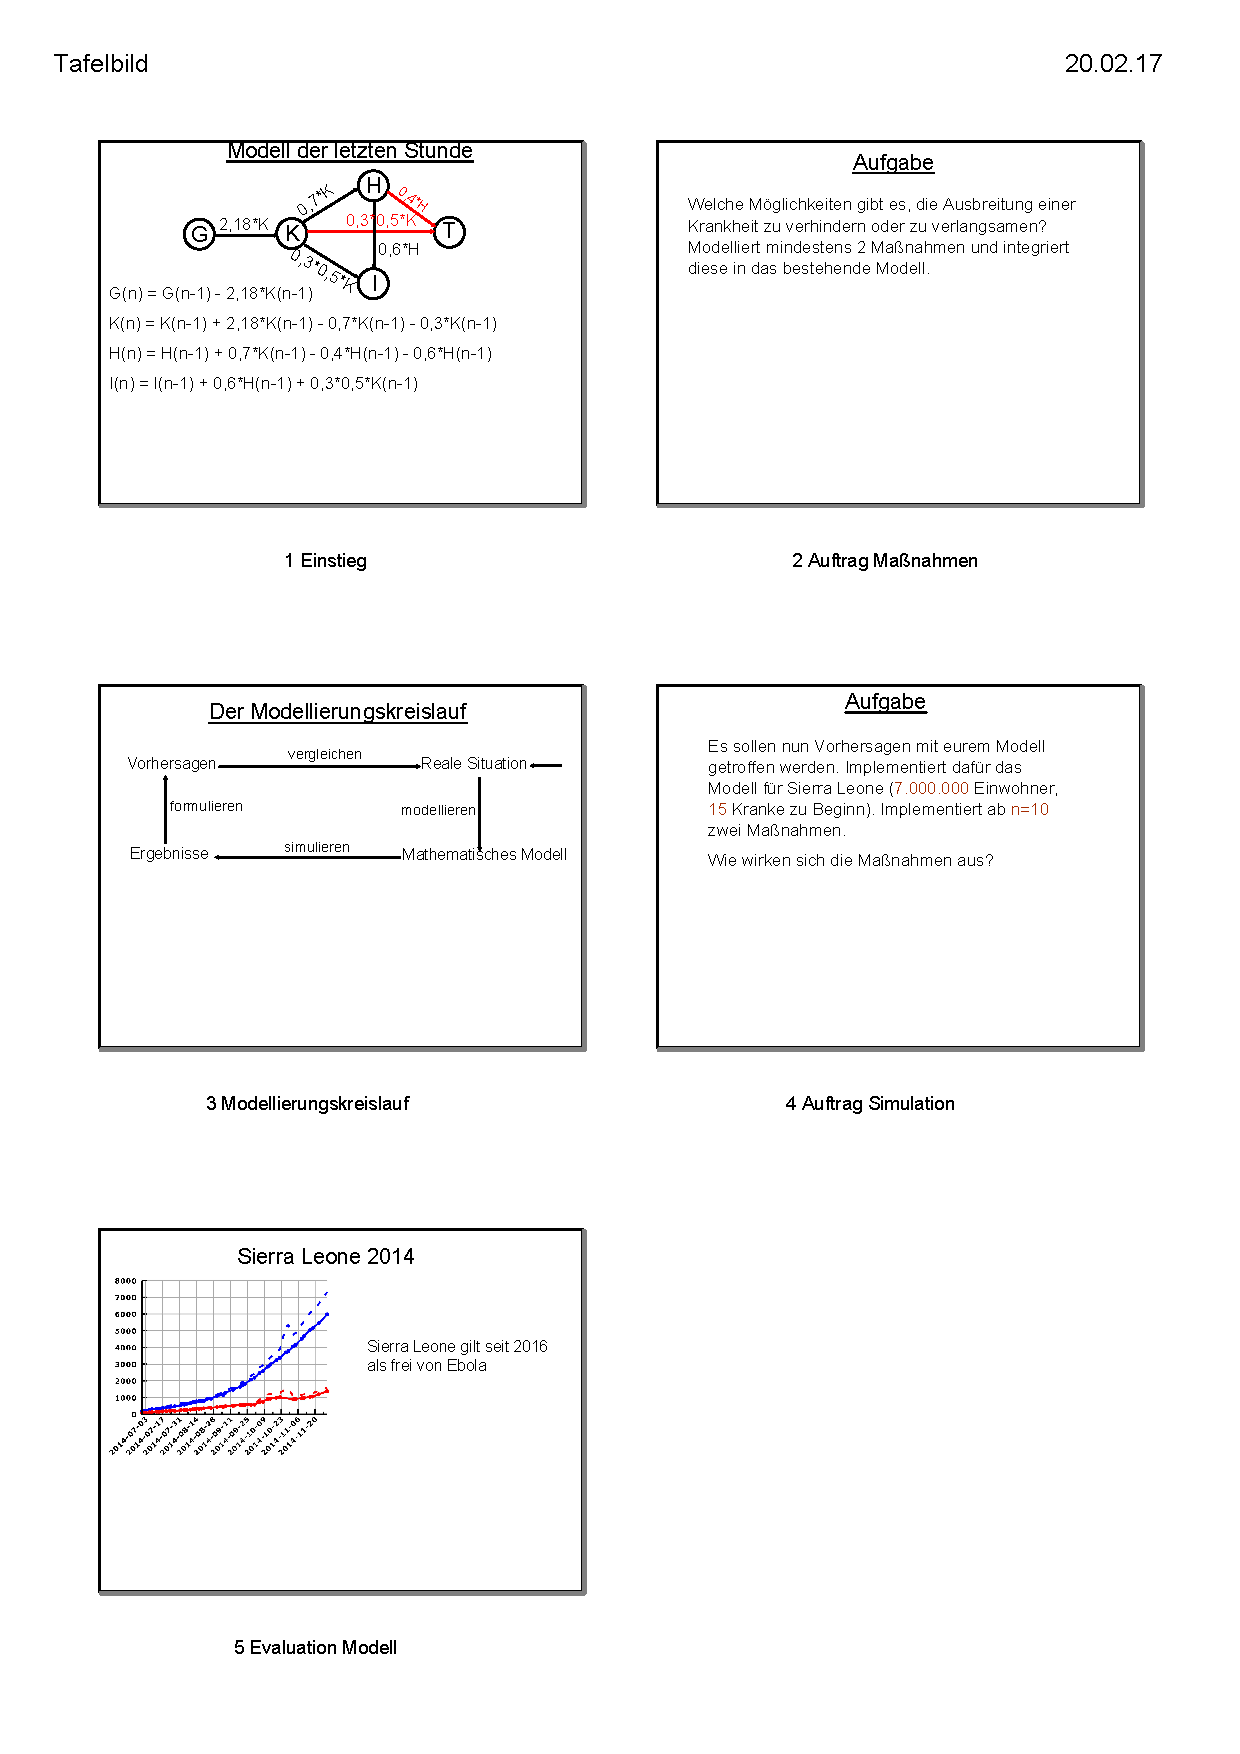
\includegraphics[width=\textwidth]{projekt/Tafelbild_3_c}
\subsubsection{Erwartungshorizont}
Bei der Einführungsaufgabe rechne ich mit keinen Schwierigkeiten. Erwartet werden Antworten wie ``Alice wird erst einmal krank, geht also in \emph{K}. Dann entscheidet sie sich entweder für oder gegen ein Krankenhaus. Sagen wir, sie geht in \emph{H}. Dort wird sie dann immun oder stirbt, geht also \emph{T} oder \emph{I}.''. Bei der Erklärung der Iterationsvorschrift für $K(n)$ erwarte ich die korrekte Zuordnung Summand zu Kante. Der Summand $K(n-1)$ sollte als ``Die, die vorher schon krank waren'' bezeichnet werden.

Bei dem ersten Arbeitsauftrag erwarte ich im Schnitt 1,5 beschriebene Maßnahmen. Eine vollständige Modellierung der Maßnahme wird nicht erwartet, wohl aber, wie sich die Maßnahme im Modell umsetzen lässt. Die Art der Maßnahmen können von gesteigerter Hygiene bis hin zu Auswanderung reichen. Bei dieser Klasse kann auch mit radikaleren und wenig sozialverträglichen Maßnahmen gerechnet werden. 

Bei dem zweiten Arbeitsauftrag werden am Ende präsentierbare Tabellenkalkulationen von fast allen Gruppen erwartet. Diese sollten mindestens eine Maßnahme ab Zeitschritt 10 umsetzen. Das Ergebnis soll von der Gruppe vorgestellt und beschrieben werden.
\subsubsection{Schülerprodukte}
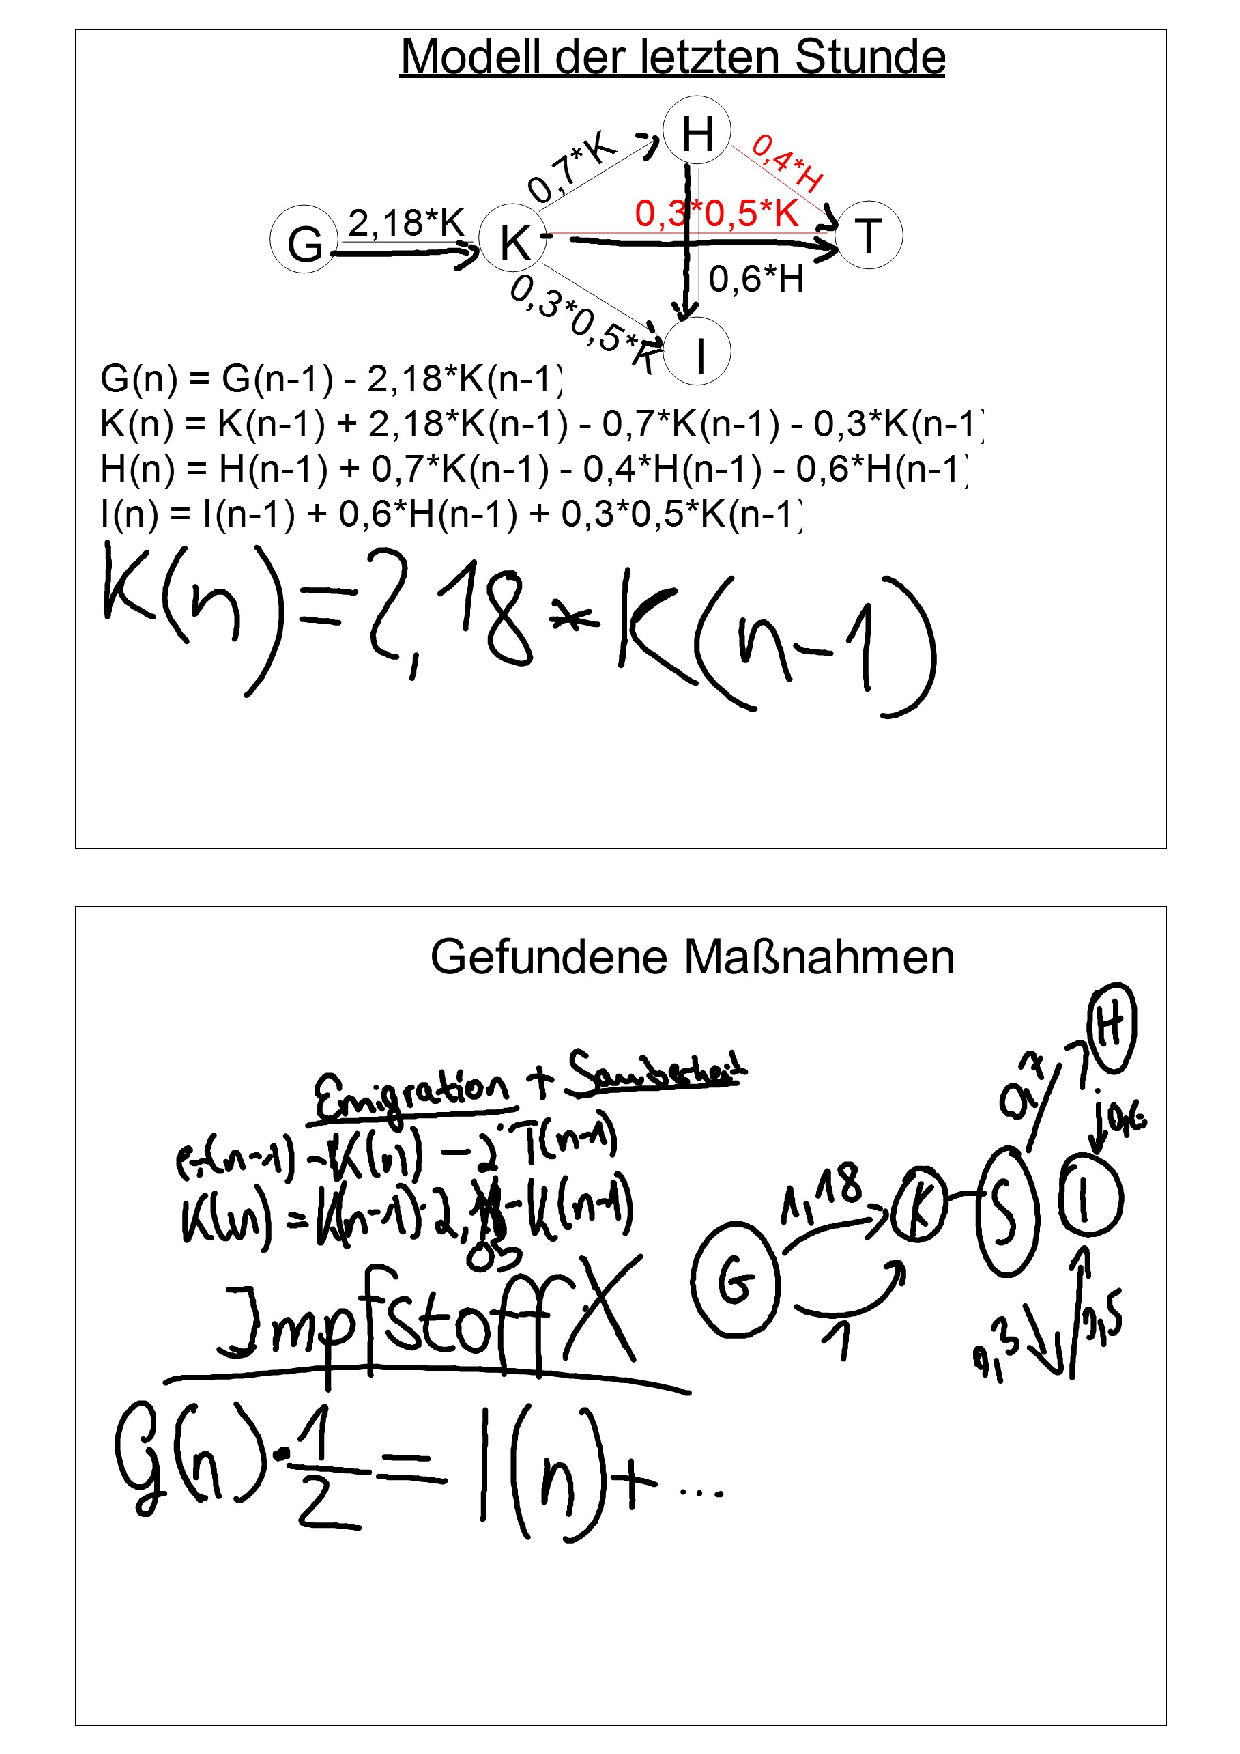
\includegraphics[width=\textwidth]{projekt/leistung_3_1}
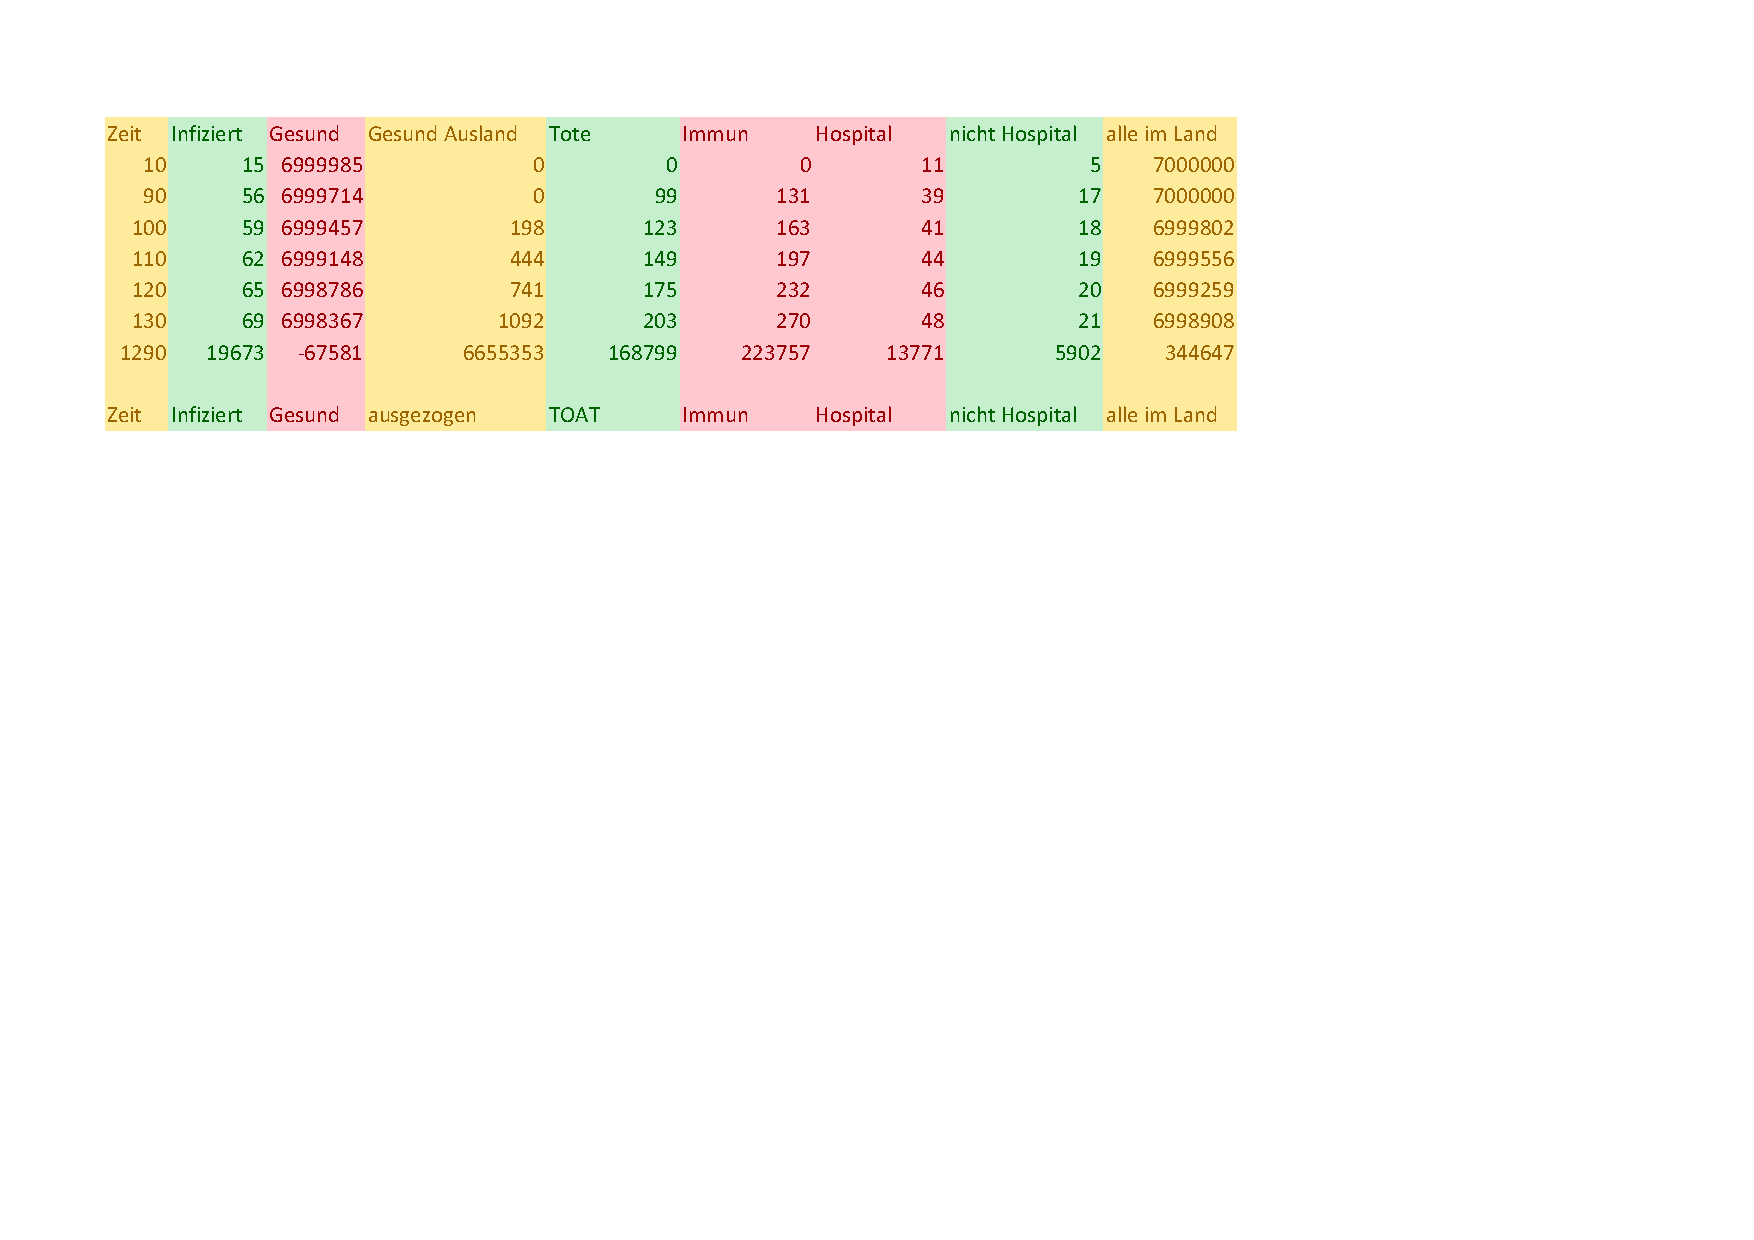
\includegraphics[width=\textwidth]{projekt/leistung_3_2}
\subsubsection{Reflexion der Stunde}
Meines Erachtens nach haben die meisten Schüler die Lernziele erreicht. Die Schüler konnten das Modell der Vorstunde erklären und Maßnahmen zur Eindämmung modellieren. Ebenso sind die verschiedenen Stadien des Modellierungskreislaufs von den Schülern verstanden und durchlaufen worden. Ausnahme bildeten 2 Schüler, die heute generell wenig Motivation zeigten. 

Ich bin der Mitarbeit der Klasse sehr zufrieden. Die Beteiligung an Fragen und Diskussionen war hoch und bisher eher ruhige Schülerinnen und Schüler haben sich eingebracht. Das handlungsorientierte Stundenkonzept wurde von der Klasse erneut gut angenommen. Die Ergebnisse, sofern vorhanden, entsprachen meinen Erwartungen an die Klasse.

Weniger zufrieden bin ich mit meiner Handhabung der weniger motivierten Schüler. Meine Versuche, die Schüler doch zur Mitarbeit zu motivieren, zeigten unterm Strich nur bei 2 von 4 Wirkung. Ein ähnlich gelagertes Problem hatte ich mit einer anderen Gruppe, die zwar motiviert mitgearbeitet, aber sich zu sehr in Details verloren hat, wodurch sie am Ende der Bearbeitungszeit des zweiten Auftrags kein fertiges Produkt vorweisen konnte. An dieser Stelle hätte ich müssen das Problem früher erkennen und entsprechend gegensteuern. Bezüglich des Vorwissens, wurde die Erfahrung der Schüler mit Excel von mir falsch eingeschätzt. Zwei Schüler hatten massive Probleme mit der Handhabung, wodurch sich in diesen beiden Fällen die oben beschriebene Demotivation erklären lässt. Die Aufwandseinschätzung des zweiten Arbeitsauftrages deckte sich nicht mit der tatsächlichen Leistung der Klasse, die meisten Gruppen haben nach 15 Minuten zusätzlicher Zeit keine verwertbaren Ergebnisse gehabt. Eine Neukonzeption der Aufgabe wäre folglich angebracht. Gleichzeitig fehlte eine Pufferaufgabe für die beiden Gruppen, die in der veranschlagten Zeit präsentierbare Ergebnisse generieren konnten. Weiterhin wurde meine Körperhaltung stellenweise als ablehnend empfunden. 

In Zukunft würde ich den Stundenaufbau im Prinzip beibehalten. Es muss aber eine bessere Analyse der Lerngruppe und deren Vorwissens erfolgen, um die Machbarkeit und den Aufwand der einzelnen Aufträge besser abschätzen zu können. Eine Reduktion der Gestaltungsfreiheit liegt auf Grund der Probleme im zweiten Auftrag nahe. Der Arbeitsauftrag könnte in kleinere Schritte aufgeteilt werden oder die Evaluation vom ersten Auftrag verbindlich für alle Gruppen festgehalten werden. Zudem muss ich an meiner Körpersprache und dem Klassenmanagement noch arbeiten. 
\subsection{Feedback der Schüler}
Am Ende der Reihe wurden die Schüler gebeten, anonym ein Feedback zur Reihe und zu deren Durchführung zu geben.